%%%%%%%%%%%%%%%%%%%%%%%%%%%%%%%%%%%%%%%%%%%%%%%%%%%%%%%%%%%%%%%%%%%%%%%%%%%%%%%
\subsection{Introduction}
%%%%%%%%%%%%%%%%%%%%%%%%%%%%%%%%%%%%%%%%%%%%%%%%%%%%%%%%%%%%%%%%%%%%%%%%%%%%%%%
\begin{frame}
 \begin{colorblock}{blue}{lightblue}{ }
    \Large \textbf{Introduction}
  \end{colorblock}
\end{frame}

\begin{frame}
\frametitle{Introduction and Objectives}
\begin{itemize}
	\item {\bf Hide the details of resource management}
	\begin{itemize}
		\item Let users instead focus on application developlemt
	\end{itemize}

\vspace{20pt}

	\item {\bf Operate applications with high reliability and availability}
	\begin{itemize}
		\item Tolerate failures within a datacenter and across datacenters
	\end{itemize}

\vspace{20pt}

	\item {\bf Run heterogeneous workloads and scale across thousands of machines}
\end{itemize}
\end{frame}

%%%%%%%%%%%%%%%%%%%%%%%%%%%%%%%%%%%%%%%%%%%%%%%%%%%%%%%%%%%%%%%%%%%%%%%%%%%%%%%
\subsection{User perspective}
%%%%%%%%%%%%%%%%%%%%%%%%%%%%%%%%%%%%%%%%%%%%%%%%%%%%%%%%%%%%%%%%%%%%%%%%%%%%%%%
\begin{frame}
 \begin{colorblock}{blue}{lightblue}{ }
    \Large \textbf{The User Perspective}
  \end{colorblock}
\end{frame}

\begin{frame}
\frametitle{Terminology}
\begin{itemize}
	\item {\bf Users develop applications called {\it jobs}}
	
\vspace{20pt}

	\item {\bf Jobs consists in one or more {\it tasks}}

\vspace{20pt}

	\item {\bf All tasks run the same binary}

\vspace{20pt}

	\item {\bf Each job runs in a set of machines managed as a unit, called a {\it Borg Cell}}
\end{itemize}
\end{frame}

\begin{frame}
\frametitle{Workloads}
\begin{itemize}
	\item {\bf Two main categories supported}
	\begin{itemize}
		\item Long-running services: jobs that should ``never'' go down, and handle short-lived, latency-sensitive requests
		\item Batch jobs: delay-tolerant jobs that can take from few seconds to few days to complete
		\item Storage services: these are long-running services like above, that are used to store data
	\end{itemize}
	\item {\bf Workload composition in a cell is dynamic}
	\begin{itemize}
		\item It varies depending on the tenants using the cell
		\item It varies with time: diurnal usage pattern for end-user-facing jobs, irregular pattern for batch jobs
	\end{itemize}
	\item {\bf Examples}
	\begin{itemize}
		\item High-priority, \texttt{production} jobs $\to$ long-running services
		\item Low-priority, \texttt{non-production} jobs $\to$ batch jobs
		\item In a typical Borg Cell
		\begin{itemize}
			\item Prod Jobs: 70\% of CPU allocation, representing 60\% of CPU usage
			\item Non-prod Jobs: 55\% of CPU allocation, representing 85\% of CPU usage
		\end{itemize}
	\end{itemize}
\end{itemize}
\end{frame}

\begin{frame}
\frametitle{Clusters and Cells}
\begin{itemize}
	\item {\bf Borg Cluster:} a set of machines connected by a high-performance datacenter-scale network fabric
	\begin{itemize}
		\item The machines in a Borg Cell all belong to a {\it single} cluster
		\item A cluster lives inside a datacenter building
		\item A collection of building makes up a {\it Site}
	\end{itemize}
	\item {\bf Borg Machines:} physical servers dedicated to execute Borg applications
	\begin{itemize}
		\item They are generally highly heterogeneous in terms of resources
		\item They may expose a public IP address
		\item They may expose advanced features, like SSD or GPGPU
	\end{itemize}
	\item {\bf Examples}
	\begin{itemize}
		\item A typical cluster usually hsts one large cell and a few small-scale test cells
		\item The {\it median cell size} is about 10 k machines
		\item Borg uses those machines to schedule application tasks, install their binaries and dependencies, monitor their health and restarting them if they fail
	\end{itemize}
\end{itemize}
\end{frame}

\begin{frame}
\frametitle{Jobs and Tasks}
\begin{itemize}
	\item {\bf Job Definition}
	\begin{itemize}
		\item Name, owner and number of tasks
		\item {\it Constraints} to force tasks run on machines with particular {\it attributes}
		\item Constraints can be {\bf hard} or {\bf soft} ({\it i.e.}, preferences)
		\item Each task maps to a set of UNIX processes running in a container on a Borg machine in a Borg Cell
	\end{itemize}

\vspace{20pt}

	\item {\bf Task Definition}
	\begin{itemize}
		\item Task index within their parent job
		\item Resource requirements
		\item Generally, all tasks have the {\it same} definition
		\item Tasks can run on {\bf any resource dimension}: there are no fixed-size slots or buckets
	\end{itemize}
\end{itemize}
\end{frame}

\begin{frame}
\frametitle{Jobs and Tasks}

\begin{itemize}
	\item {\bf The Borg Configuration Language}
	\begin{itemize}
		\item Declarative language to specify jobs and tasks
		\item Lambda functions to allow calculations
		\item Some application descriptions can be over 1 k lines of code
	\end{itemize}

\vspace{20pt}

	\item {\bf User interacting with live jobs}
	\begin{itemize}
		\item This is achieved mainly using RPC
		\item Users can update the specification of tasks, while their parent job is running
		\item Updates are non-atomic, executed in a rolling-fashion
	\end{itemize}

\vspace{20pt}

	\item {\bf Task updates ``side-effects''}
	\begin{itemize}
		\item Always require restarts: e.g., pushing a new binary
		\item Might require migration: e.g., change in specification
		\item Never require restarts nor migrations: e.g., change in priority
	\end{itemize}
\end{itemize}
\end{frame}

\begin{frame}
\frametitle{Jobs State Diagram}
\begin{figure}[h]
  \centering
  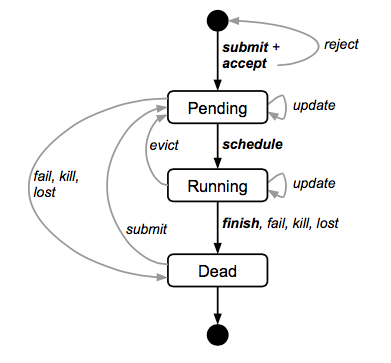
\includegraphics[scale=0.5]{./figures/borg_state_diagram}
  \label{fig:borg_state_diagram}
\end{figure}
\end{frame}

\begin{frame}
\frametitle{Resource Allocations}
\begin{itemize}
	\item {\bf The Borg ``Alloc''}
	\begin{itemize}
		\item Reserved set of resources on {\bf an individual machine}
		\item Can be used to execute one or more tasks, that equally share resources
		\item {\bf Resources remain assigned whether or not they are used}
	\end{itemize}

\vspace{20pt}

	\item {\bf Typical use of Borg Allocs}
	\begin{itemize}
		\item Set resources aside for future tasks
		\item Retain resources between stopping and starting tasks
		\item Consolidate (gather) tasks from different jobs on the same machine
	\end{itemize}

\vspace{20pt}

	\item {\bf Alloc Sets}
	\begin{itemize}
		\item Group of allocs on different machines
		\item Once an alloc set has been created, one or more jobs can be submitted
	\end{itemize}
\end{itemize}
\end{frame}

\begin{frame}
\frametitle{Priority, Quota and Admission Control}
\begin{itemize}
	\item {\bf Mechanisms to deal with resource demand and offer}
	\begin{itemize}
		\item What to do when more work shows up than can be accommodated?
		\item Note: this is not {\it scheduling}, it is more admission control
	\end{itemize}
	\item {\bf Job priority}
	\begin{itemize}
		\item Non-overlapping {\it priority bands} for different uses
		\item This essentially means users must ``manually'' cluster their applications according to such bands
		\item[$\to$] Tasks from high-priority jobs can preempt low-priority tasks
		\item Cascade preemption is avoided by disabling it for same-band jobs
	\end{itemize}
	\item {\bf Job/User quotas}
	\begin{itemize}
		\item Used to decide which job to admit for scheduling
		\item Expressed as a vector of resource quantities
	\end{itemize}
	\item {\bf Pricing}
	\begin{itemize}
		\item Underlying mechanism to regulate user behavior
		\item Aligns user incentives to better resource utilization
		\item Discourages over-buying by over-selling quotas at lower priority
	\end{itemize}
\end{itemize}
\end{frame}

\begin{frame}
\frametitle{Naming Services}
\begin{itemize}
	\item {\bf Borg Name Service}
	\begin{itemize}
		\item A mechanism to assign a name to tasks
		\item Task name = Cell name, job name and task number
	\end{itemize}

\vspace{20pt}

	\item {\bf Uses the Chubby coordination service}
	\begin{itemize}
		\item Writes task names into it
		\item Writes also health information and status
		\item Used by Borg RPC mechanism to establish communication endpoints
	\end{itemize}

\vspace{20pt}

	\item {\bf DNS service inherits from BNS}
	\begin{itemize}
		\item Example: the 50th task in job ``jfoo'' owned by user ``ubar'' in a Borg Cell called ``cc''
		\item \texttt{50.jfoo.ubar.cc.borg.google.com}
	\end{itemize}
\end{itemize}
\end{frame}

\begin{frame}
\frametitle{Monitoring Services}
\begin{itemize}
	\item {\bf Every task in Borg has a built-in HTTP server}
	\begin{itemize}
		\item Provides health information
		\item Provides performance metrics
	\end{itemize}
	\item {\bf Borg SIGMA}
	\begin{itemize}
		\item Monitoring UI Service
		\item State of jobs, of cells
		\item Drill-down to task level
		\item {\bf Why pending?}
		\begin{itemize}
			\item ``Debugging'' service
			\item Helps users with finding job specifications that can be easily scheduled
		\end{itemize}
	\end{itemize}
	\item {\bf Billing services}
	\begin{itemize}
		\item Use monitoring information to compute usage-based charging
		\item Help users debug their jobs
		\item Used for capacity planning
	\end{itemize}
\end{itemize}
\end{frame}

%%%%%%%%%%%%%%%%%%%%%%%%%%%%%%%%%%%%%%%%%%%%%%%%%%%%%%%%%%%%%%%%%%%%%%%%%%%%%%%
\subsection{Borg Architecture}
%%%%%%%%%%%%%%%%%%%%%%%%%%%%%%%%%%%%%%%%%%%%%%%%%%%%%%%%%%%%%%%%%%%%%%%%%%%%%%%
\begin{frame}
 \begin{colorblock}{blue}{lightblue}{ }
    \Large \textbf{Borg Architecture}
  \end{colorblock}
\end{frame}

\begin{frame}
\frametitle{Architecture Overview}
\begin{figure}[h]
  \centering
  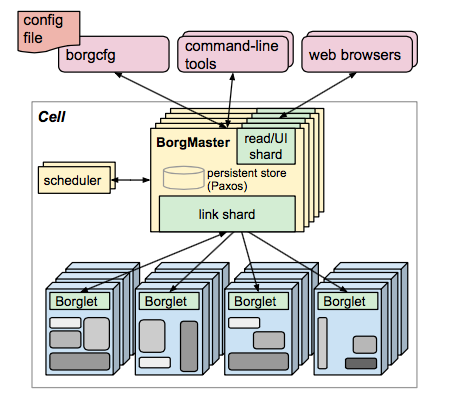
\includegraphics[scale=0.5]{./figures/borg_architecture}
  \label{fig:borg_arch}
\end{figure}
\end{frame}

\begin{frame}
\frametitle{Architecture Overview}
\begin{itemize}
	\item {\bf Architecture components}
	\begin{itemize}
		\item A set of physical machines
		\item A {\it logically centralized} controller, the {\bf Borgmaster}
		\item An agent process running on all machines, the {\bf Borglet}
	\end{itemize}
\end{itemize}
\end{frame}

\begin{frame}
\frametitle{The Borgmaster: Components}
\begin{itemize}
	\item {\bf The Borgmaster}
	\begin{itemize}
		\item One per Borg Cell
		\item Orchestrates cell resources
	\end{itemize}

\vspace{20pt}

	\item {\bf Components}
	\begin{itemize}
		\item The Borgmaster process
		\item The scheduler process
	\end{itemize}

\vspace{20pt}

	\item {\bf The Borgmaster process}
	\begin{itemize}
		\item Handles client RPCs that either mutate state or lookup for state
		\item Manages the state machines for all Borg ``objects'' (machines, tasks, allocs, etc...)
		\item Communicates with all Borglets in the cell
		\item Provides a Web-based UI
	\end{itemize}
\end{itemize}
\end{frame}

\begin{frame}
\frametitle{The Borgmaster: Reliability}
\begin{itemize}
	\item {\bf Borgmaster reliability achieved through replication}
	\begin{itemize}
		\item Single logical process, replicated 5 times in a cell
		\item Single master elected using Paxos when starting a cell, or upon failure of the current master
		\item Master serves as Paxos leader and cell state mutator
	\end{itemize}

\vspace{20pt}

	\item {\bf Borgmaster replicas}
	\begin{itemize}
		\item Maintain an {\bf in-memory} fresh copy of the cell state
		\item Persist their state to a distributed Paxos-based store
		\item Help building the most up-to-date cell state when a new master is elected
	\end{itemize}
\end{itemize}
\end{frame}

\begin{frame}
\frametitle{The Borgmaster: State}
\begin{itemize}
	\item {\bf Borgmaster checkpoints its state}
	\begin{itemize}
		\item Time-based and event-based mechanism
		\item State include everything related to a cell
	\end{itemize}

\vspace{20pt}

	\item {\bf Checkpoint utilization}
	\begin{itemize}
		\item Restore the state to a functional one, e.g. before a failure or a bug
		\item Studying a faulty state a fixing it by hand
		\item Build a persistent log of events for future queries
		\item Use it for offline simulations
	\end{itemize}
\end{itemize}
\end{frame}

\begin{frame}
\frametitle{The Fauxmaster}
\begin{itemize}
	\item {\bf A high-fidelity simulator}
	\begin{itemize}
		\item It reads checkpoint files
		\item Full-fledged Borgmaster code
		\item Stubbed-out interfaces to Borglets
	\end{itemize}
	\item {\bf Fauxmaster operation}
	\begin{itemize}
		\item Accepts RPCs to make state machine changes
		\item Connects to simulated Borglets that replay real interactions from checkpoint files
	\end{itemize}
	\item {\bf Fauxmaster benefits}
	\begin{itemize}
		\item Help users debug their application
		\item Capacity planning, e.g. ``How many new jobs of this type would fit in the cell?''
		\item Perform sanity checks for cell configurations, e.g. ``Will this new configuration evict any important jobs?''
	\end{itemize}
\end{itemize}
\end{frame}

\begin{frame}
\frametitle{Scheduling}
\begin{itemize}
	\item {\bf Queue based mechanism}
	\begin{itemize}
		\item New submitted jobs (and their tasks) are stored in the Paxos store (for reliability) and put in the {\it pending queue}
	\end{itemize}
	\item {\bf The scheduler process}
	\begin{itemize}
		\item {\color{red} Operates at the task level, not the job level}
		\item Scans {\bf asynchronously} the pending queue
		\item Assigns tasks to machines that satisfy constraints and that have enough resources
	\end{itemize}
	\item {\bf Pending task selection}
	\begin{itemize}
		\item Scanning proceeds from high to low priority tasks
		\item Within the same priority class, scheduling uses a round-robin mechanism
		\item[$\to$] Ensures fairness
		\item[$\to$] Avoids head-of-line blocking behind large jobs
	\end{itemize}
\end{itemize}
\end{frame}

\begin{frame}
\frametitle{Scheduling Algorithm}
\begin{itemize}
	\item {\bf The scheduling algorithm has two main processes}

\vspace{20pt}

	\begin{itemize}
		\item {\bf Feasibility checking}: find a set of machines that
		\begin{itemize}
		 	\item Meet tasks' constraints
		 	\item Have enough available resources, including those that are currently assigned to low-priority tasks that can be evicted
		 \end{itemize}

\vspace{20pt}

		\item {\bf Scoring}: among the set returned by the previous process, rank such machines to
		\begin{itemize}
			\item Minimize the number and priority of preempted tasks
			\item Prefer machines with a local copy of tasks binaries and dependencies
			\item Spread tasks across failure and power domains
			\item Pack and spread tasks, mixing high and low priority ones on the same machine to allow high-priority tasks to eventually expand
		\end{itemize}
	\end{itemize}
\end{itemize}
\end{frame}

\begin{frame}
\frametitle{More on the scoring mechanism}
\begin{itemize}
	\item {\bf Worst-fit scoring: spreading tasks}
	\begin{itemize}
		\item Single cost value across heterogeneous resources
		\item Minimize the change in cost when placing a new task
		\item[$\to$] Leaves headroom for load spikes
		\item[$\to$] But leads to fragmentation
	\end{itemize}

\vspace{20pt}

	\item {\bf Best-fit scoring: ``waterfilling'' algorithm}
	\begin{itemize}
		\item Tries to fill machines as tightly as possible
		\item[$\to$] Leaves empty machines that can be used to place large tasks
		\item[$\to$] But difficult to deal with load spikes as the headroom left in each machine depends highly on load estimation
	\end{itemize}

\vspace{20pt}

	\item {\bf Hybrid}
	\begin{itemize}
		\item Tries to reduce the amount of stranded resources
		\item Performs better than best-fit
	\end{itemize}
\end{itemize}
\end{frame}

\begin{frame}
\frametitle{Task startup latency}
\begin{itemize}
	\item {\bf Task startup latency is a very important metric to optimize}
	\begin{itemize}
		\item Time from job submission to a task running
		\item Highly variable
		\item Median is about 25 s
	\end{itemize}

\vspace{20pt}

	\item {\bf Techniques to reduce latency}
	\begin{itemize}
		\item The main culprit for high latency is binary and package installations
		\item Idea: place tasks on machines that already have dependencies installed
		\item Packages and binaries distributed using a BitTorrent-like protocol
	\end{itemize}
\end{itemize}
\end{frame}

\begin{frame}
\frametitle{The Borglet}
\begin{itemize}
	\item {\bf The Borglet}
	\begin{itemize}
		\item Borg agent present on every machine in a cell
		\item Starts and stop tasks
		\item Restarts failed tasks
		\item Manages machine resources interacting with the OS
		\item Maintains and rolls over debug logs
		\item Report the state of the machine to the Borgmaster
	\end{itemize}

\vspace{20pt}

	\item {\bf Interaction with the Borgmaster}
	\begin{itemize}
		\item Pull-based mechanism: heartbeat-like messages every few seconds
		\item[$\to$] Borgmaster perform flow and rate control to avoid message storms
		\item Borglet continues operation even if communication to Borgmaster is interrupted
		\item A failed Borglet is blacklisted and all tasks are rescheduled
	\end{itemize}
\end{itemize}
\end{frame}

\begin{frame}
\frametitle{Borglet to Borgmaster communication}
\begin{itemize}
	\item {\bf How to handle control message overhead?}
	\begin{itemize}
		\item Many Borgmaster replicas receive state updates
		\item Many Borglets communicate concurrently
	\end{itemize}

\vspace{20pt}

	\item {\bf The link shard mechanism}
	\begin{itemize}
		\item Each borgmaster replica communicates with a subset of the cell Borglets
		\item Partitioning is computed at each leader election
		\item Borglets report full state, but the link shard mechanism aggregate state information
		\item[$\to$] Differential state update, to reduce the load at the master
	\end{itemize}
\end{itemize}
\end{frame}

\begin{frame}
\frametitle{Scalability}
\begin{itemize}
	\item {\bf A typical Borgmaster resource requirements}
	\begin{itemize}
		\item Manages 1000s of machines in a cell
		\item Arrival rates of 10,000 tasks per minute
		\item 10+ cores, 50+ GB of RAM
	\end{itemize}

\vspace{20pt}

	\item {\bf Decentralized design}
	\begin{itemize}
		\item Scheduler process separate from Borgmaster process
		\item One scheduler per Borgmaster replica
		\item Scheduling is somehow decentralized
		\item State change communicated from replicas to elected Borgmaster, that finalizes the state update
	\end{itemize}

\vspace{20pt}

	\item {\bf Additional techniques to achieve scalability}
	\begin{itemize}
		\item Score caching
		\item Equivalence class
		\item Relaxed randomization
	\end{itemize}
\end{itemize}
\end{frame}

%%%%%%%%%%%%%%%%%%%%%%%%%%%%%%%%%%%%%%%%%%%%%%%%%%%%%%%%%%%%%%%%%%%%%%%%%%%%%%%
\subsection{Borg Behavior}
%%%%%%%%%%%%%%%%%%%%%%%%%%%%%%%%%%%%%%%%%%%%%%%%%%%%%%%%%%%%%%%%%%%%%%%%%%%%%%%
\begin{frame}
 \begin{colorblock}{blue}{lightblue}{ }
    {\Large \textbf{Borg Behavior: Experimental Perspective}}

    Also, additional details on how Borg works...
  \end{colorblock}
\end{frame}

\begin{frame}
\frametitle{Availability}
\begin{itemize}
	\item {\bf In large scale systems, failure are the norm not the exception}
	\begin{itemize}
		\item Everything can fail, and both Borg and its running applications must deal with this
	\end{itemize}
	\item {\bf Baseline techniques to achieve high availability}
	\begin{itemize}
		\item Replication
		\item Storing persistent state in a distributed file system
		\item Checkpointing
	\end{itemize}
	\item {\bf Additional techniques}
	\begin{itemize}
		\item Automatic rescheduling of failed tasks
		\item Mitigating correlated failures
		\item Rate limitation
		\item Avoid duplicate computation
		\item Admission control to avoid overload
		\item Minimize external dependencies for task binaries
	\end{itemize}
\end{itemize}
\begin{figure}[h]
  \centering
  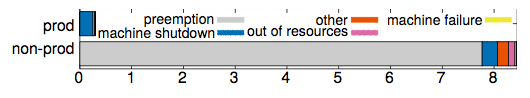
\includegraphics[scale=0.5]{./figures/borg_eviction_causes}
  \label{fig:borg_eviction_causes}
\end{figure}

\end{frame}

\begin{frame}
\frametitle{System Utilization}
\begin{itemize}
	\item {\bf The primary goal of a cluster scheduler is to achieve high utilization}
	\begin{itemize}
		\item Machines, network fabric, power, cooling ... represent a significant financial investment
		\item Increasing utilization by a few percent can save millions!
	\end{itemize}
	\item {\bf A sophisticated metric: Cell Compaction}
	\begin{itemize}
		\item Replaces the typical ``average utilization'' metric
		\item Provides a fair, consistent way to compare scheduling policies
		\item Translates directly into cost/benefit result
		\item Computed as follows:
		\begin{itemize}
			\item Given a workload in a point in time (so this is not trace driven simulation)
			\item Enter a loop of workload packing
			\item At each iteration, remove physical machines from the cell
			\item Exit the loop when the workload can no longer fit the cell size
		\end{itemize}
	\end{itemize}
	\item {\bf Use the Fauxmaster to produce experimental results}
\end{itemize}
\end{frame}

\begin{frame}
\frametitle{System Utilization: Compaction}
\begin{figure}[h]
  \centering
  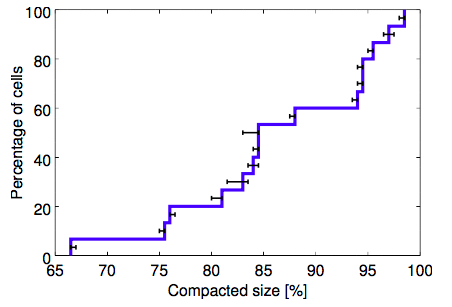
\includegraphics[scale=0.4]{./figures/borg_exp_utilization}
  \label{fig:borg_exp_utilization}
\end{figure}
\begin{itemize}
	\item This graphs shows how much smaller cells would be if we applied compaction to them
\end{itemize}
\end{frame}

\begin{frame}
\frametitle{System Utilization: Cell Sharing}
\begin{itemize}
	\item {\bf Fundamental question: to share or not to share?}
	\begin{itemize}
		\item Many current systems apply static partitioning: one cluster {\bf dedicated only} to prod jobs, one cluster for non-prod jobs
	\end{itemize}
	\item {\bf Benefits from sharing}
	\begin{itemize}
		\item Borg can reclaim resources reserved by ``anxious'' prod jobs 
	\end{itemize}
\end{itemize}
\begin{figure}[h]
  \centering
  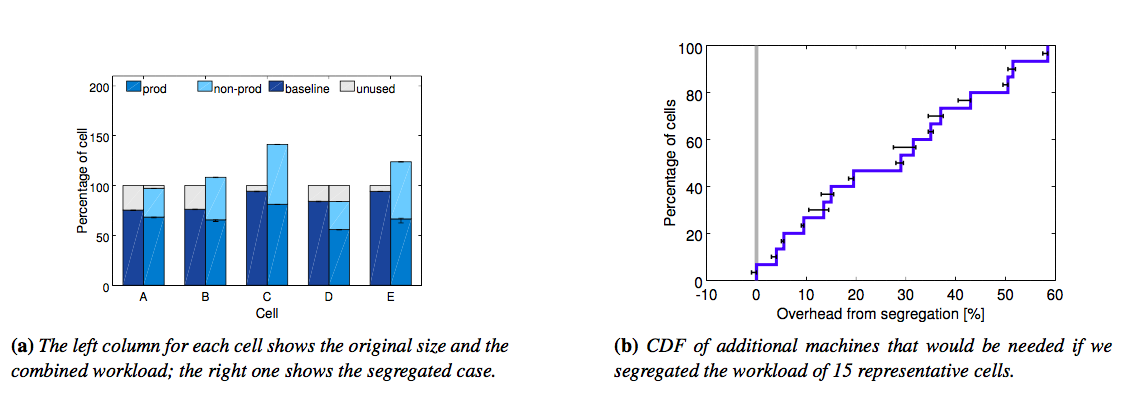
\includegraphics[scale=0.3]{./figures/borg_exp_sharing}
  \label{fig:borg_exp_sharing}
\end{figure}
\end{frame}

\begin{frame}
\frametitle{System Utilization: Cell Sizing}
\begin{itemize}
	\item {\bf Fundamental question: large or small cells?}
	\begin{itemize}
		\item Large cells to accommodate large jobs
		\item Large cells also avoid fragmentation
	\end{itemize}
\end{itemize}
\begin{figure}[h]
  \centering
  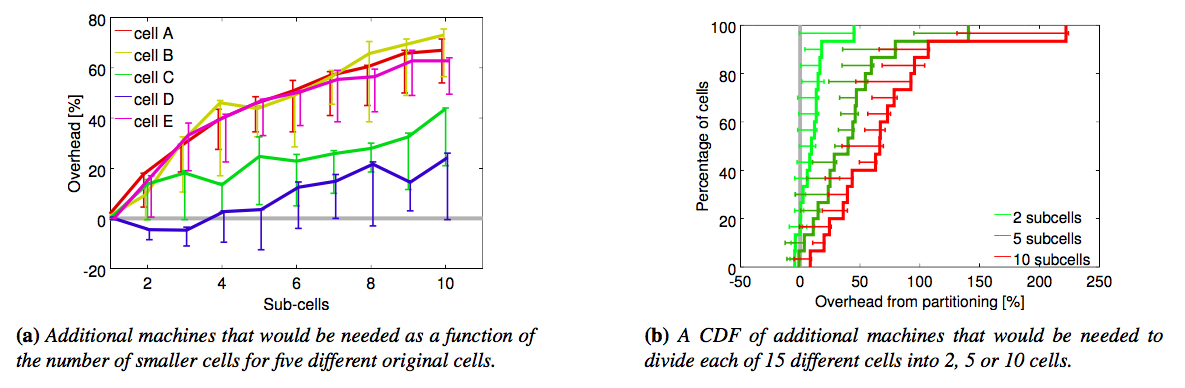
\includegraphics[scale=0.3]{./figures/borg_exp_size}
  \label{fig:borg_exp_size}
\end{figure}
\end{frame}

\begin{frame}
\frametitle{System Utilization: Fine-grained Resource Requests}
\begin{itemize}
	\item {\bf Borg users specify Job requirements in terms of resources}
	\begin{itemize}
		\item For CPU: this is done in milli-core
		\item For RAM and disk: this is done in bytes
	\end{itemize}
\end{itemize}
\begin{figure}[h]
  \centering
  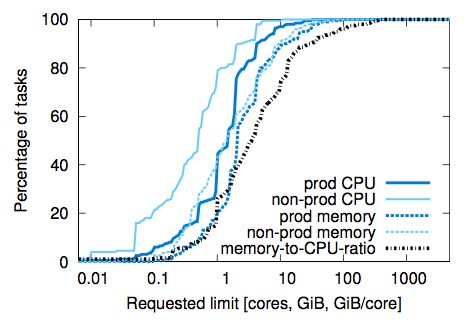
\includegraphics[scale=0.4]{./figures/borg_exp_fine}
  \label{fig:borg_exp_size}
\end{figure}
\end{frame}

\begin{frame}
\frametitle{System Utilization: Fine-grained Resource Requests}
\begin{itemize}
	\item {\bf Would fixed size containers (or slot) be good?}
	\begin{itemize}
		\item No! It would require more machines in a cell!
	\end{itemize}
\end{itemize}
\begin{figure}[h]
  \centering
  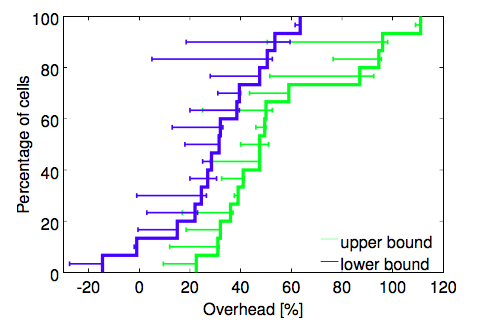
\includegraphics[scale=0.4]{./figures/borg_exp_bucket}
  \label{fig:borg_exp_size}
\end{figure}
\end{frame}

\begin{frame}
\frametitle{System Utilization: Resource Reclamation}
\begin{itemize}
	\item {\bf Borg users specify resource {\it limits} for their jobs}
	\begin{itemize}
		\item Used to perform admission control
		\item Used for feasibility checking ({\it i.e.,} find sets of suitable machines in a cell)
	\end{itemize}
	\item {\bf Borg users have the tendency to ``over provision'' for their jobs}
	\begin{itemize}
		\item Some tasks, occasionally need to use all their resources
		\item Most of the tasks never use all resources
	\end{itemize}
	\item {\bf Resource reclamation}
	\begin{itemize}
		\item Borg builds estimates of resource usage: these are called {\bf resource reservations}
		\item Borgmaster receives usage updates from Borglets
		\item Prod jobs are treated differently: they do not rely on reclaimed resources, Borgmaster only uses resource limits
	\end{itemize}
\end{itemize}
\end{frame}

\begin{frame}
\frametitle{System Utilization: Resource Reclamation}
\begin{figure}[h]
  \centering
  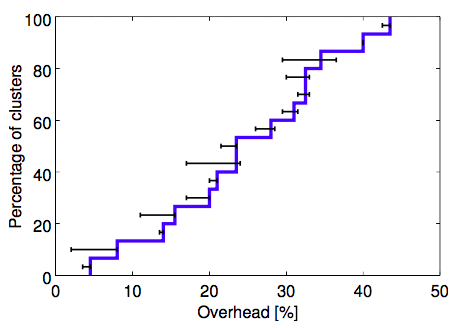
\includegraphics[scale=0.4]{./figures/borg_exp_reclamation1}
  \label{fig:borg_exp_reclamation1}
\end{figure}
\begin{itemize}
	\item Resource reclamation is quite effective. A CDF of the additional machines that would be needed if it was disabled.
\end{itemize}
\end{frame}

\begin{frame}
\frametitle{System Utilization: Resource Reclamation}
\begin{figure}[h]
  \centering
  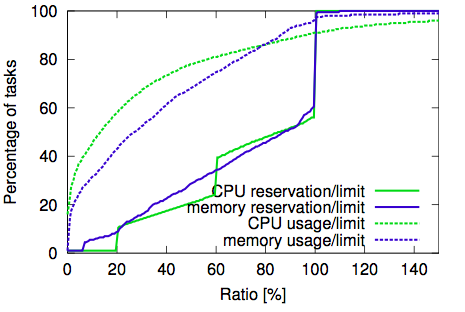
\includegraphics[scale=0.4]{./figures/borg_exp_reclamation2}
  \label{fig:borg_exp_reclamation2}
\end{figure}
\begin{itemize}
	\item Resource estimation is successful at identifying unused resources. Most tasks use much less than their limit, although a few use more CPU than requested.
\end{itemize}
\end{frame}

\begin{frame}
\frametitle{Isolation}
\begin{itemize}
	\item {\bf Sharing a multi-tenancy are beneficial, but...}
	\begin{itemize}
		\item Tasks may interfere one with each other
		\item Need a good mechanism to prevent interference (both in terms of security and performance)
	\end{itemize}
	\item {\bf Performance isolation}
	\begin{itemize}
		\item All tasks run in Linux cgroup-based containers
		\item Borglets operate on the OS to control container resources
		\item A control-loop assigns resources based on predicted future usage or on memory pressure
	\end{itemize}
	\item {\bf Additional techniques}
	\begin{itemize}
		\item Application classes: latency-sensitive, vs. batch
		\item Resource classes: compressible and non-compressible
		\item Tuning of the underlying OS, especially the OS scheduler
	\end{itemize}
\end{itemize}
\end{frame}

%%%%%%%%%%%%%%%%%%%%%%%%%%%%%%%%%%%%%%%%%%%%%%%%%%%%%%%%%%%%%%%%%%%%%%%%%%%%%%%
\subsection{Lessons Learned}
%%%%%%%%%%%%%%%%%%%%%%%%%%%%%%%%%%%%%%%%%%%%%%%%%%%%%%%%%%%%%%%%%%%%%%%%%%%%%%%
\begin{frame}
 \begin{colorblock}{blue}{lightblue}{ }
    {\Large \textbf{Lessons learned from building and operating Borg}}

    And what has been included in Kubernetes, the open source version of Borg...
  \end{colorblock}
\end{frame}

\begin{frame}\frametitle{Lessons Learned: the Bad}
\begin{itemize}
	\item {\bf The ``job'' abstraction is too simplistic}
	\begin{itemize}
		\item Multi-job services cannot be easily managed, nor addressed
		\item Kubernetes uses scheduling units called {\bf pods} ({\it i.e.,} the Borg allocs) and {\bf labels} (key/value pairs describing objects)
	\end{itemize}
	\item {\bf Addressing services is critical}
	\begin{itemize}
		\item One IP address implies managing ports as a resource, which complicates tasks
		\item Kubernetes uses Linux name-spaces, such that each pod has its own IP address
	\end{itemize}
	\item {\bf Power or casual users?}
	\begin{itemize}
		\item Borg is geared toward power users: e.g., BCL has about 230 parameters!
		\item Build automation tools, and template settings from historical executions
	\end{itemize}
\end{itemize}
\end{frame}

\begin{frame}\frametitle{Lessons Learned: the Good}
\begin{itemize}
	\item {\bf Allocs are useful}
	\begin{itemize}
		\item Resource envelope for one or more container co-scheduled on the same machine and that can share resources
	\end{itemize}
	\item {\bf Cluster management is more than task management}
	\begin{itemize}
		\item Naming and load balancing are first-class citizens
	\end{itemize}
	\item {\bf Introspection is vital}
	\begin{itemize}
		\item Clearly true for debugging
		\item Key for capacity planning and monitoring
	\end{itemize}
	\item {\bf The master is the kernel of a distributed system}
	\begin{itemize}
		\item Monolithic designs are not working well
		\item Cooperation of micro-services that use a common low-level API to process requests and manipulate state
	\end{itemize}
\end{itemize}
\end{frame}
